\documentclass{article}
\usepackage{amsmath}
\usepackage[margin=1in]{geometry}
\usepackage{amsfonts}
\usepackage{hyperref}
\usepackage{graphicx}


\begin{document}
	
\title{Dot and Cross Products}
\author{Andy Chong Sam}

\maketitle	

\section {The Law of Cosines}

\par\noindent We start with the derivation of the law of cosines:

\begin{flalign}
c^{2} = a^{2} + b^{2} -2ab\cos(C)
\end{flalign} 

\begin{minipage}[c]{.6\linewidth}
		
	\begin{flalign*}
		\overline{CD} = a\cos{C} \\
		\overline{DA} = b- a\cos{C} \\
		\overline{BD} = a\sin{C} \\ \\	
		c^{2} = (\overline{BD})^{2} + (\overline{DA})^{2} \\
		= (a\sin{C})^{2} + (b- a\cos{C})^{2} \\
		= a^{2}\sin^{2}{C} + a^{2}cos^{2}{C} + b^{2} -2ab\cos(C) \\
		= a^{2}(\sin^2{C} + \cos^2{C}) + b^{2} -2ab\cos(C) \\
		= a^{2} + b^{2} -2ab\cos(C) \\	
	\end{flalign*}



\end{minipage}%%%
\begin{minipage}[c]{.4\linewidth}
\begin{center}
	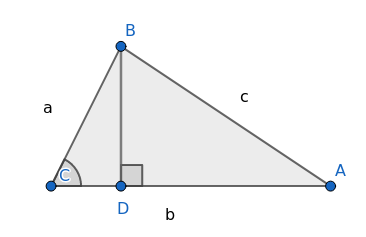
\includegraphics[width=7cm]{dot-cross-1.png}
\end{center}
\begin{center}
	Figure 1	
\end{center}
\end{minipage}

\par\noindent We can restate the law of cosines in terms of vectors and derive this expression:

\begin{flalign}
\vec{a}\cdot\vec{b} = ||\vec{a}||\;||\vec{b}||\cos\theta
\end{flalign}
 
\begin{minipage}{.6\linewidth}
	
		\par\noindent First, we restate expression (1) in terms of vectors. 
		
	\begin{flalign*}
		|| \vec{a} -\vec{b}||^{2} = ||\vec{a}||^{2} + ||\vec{b}||^{2} - 2 ||\vec{a}||\;||\vec{b}||\cos\theta \\
	\end{flalign*}

		\par\noindent  We can restate the left hand side using the fact that the dot product of a vector with itself is its squared magnitude:

    \begin{flalign*}	
		|| \vec{a} - \vec{b}||^{2} = ( \vec{a} - \vec{b}) \cdot ( \vec{a} - \vec{b}) \\ 	
		= \vec{a}\cdot\vec{a} - 2(\vec{a}\cdot\vec{b}) + \vec{b}\cdot\vec{b}
		= ||\vec{a}||^{2} - 2(\vec{a}\cdot\vec{b}) + ||\vec{b}||^{2}
	\end{flalign*}

	\par\noindent Now we substitute this result back into the left hand side of the original expression:
	
		\begin{flalign*}
			||\vec{a}||^{2} - 2(\vec{a}\cdot\vec{b}) + ||\vec{b}||^{2} = ||\vec{a}||^{2} + ||\vec{b}||^{2} - 2 ||\vec{a}||\;||\vec{b}||\cos\theta  \\
			\vec{a}\cdot\vec{b} = |\vec{a}||\;||\vec{b}||\cos\theta	
		\end{flalign*}

\end{minipage}
\begin{minipage}[c]{.4\linewidth}
	\begin{center}
		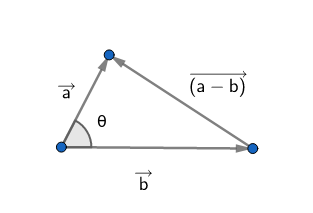
\includegraphics[width=7cm]{dot-cross-2.png}		
	\end{center}
	\begin{center}
		Figure 2	
	\end{center}
	
	
\end{minipage}

\newpage
\section {Projection}

\begin{minipage}{.6\linewidth}
	\par\noindent A useful feature of the dot product is that it assists with calculating vector projection. In Figure 3 we have the length w, which is the projection of \(\vec{a}\) onto \(\vec{b}\). We can start with the definition of w with respect to \(cos\theta\) and the magnitude of \(\vec{a}\):
	\begin{flalign*}
		w= \cos\theta ||\vec{a}|| \\	
	\end{flalign*}	

	\par\noindent We know from expression (2) that \(\cos\theta=\frac{\vec{a}\cdot\vec{b}}{||\vec{a}||\;||\vec{b}||}\). Substituting this into the equation for w, we get:
	
	\begin{flalign*}
		w= \frac{\vec{a}\cdot\vec{b}\;||\vec{a}||}{||\vec{a}||\;||\vec{b}||} \\
		w= \frac{\vec{a}\cdot\vec{b}}{||\vec{b}||}
	\end{flalign*}
\end{minipage}
\begin{minipage}[c]{.4\linewidth}
		\begin{center}
		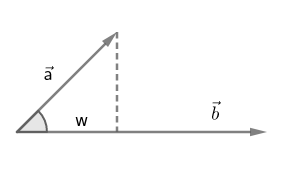
\includegraphics[width=7cm]{dot-cross-3.png}		
	\end{center}
	\begin{center}
		Figure 2	
	\end{center}
\end{minipage}

\section {The Dot Product of Orthogonal Vectors}

\par\noindent The dot product of two orthogonal (perpendicular) vectors is zero. Suppose again that we have two vectors \( \vec{a} \) and \( \vec{b} \), and they are perpendicular to each other, then the angle \( \theta\) between them is \( \frac{\pi}{2}\). This results in the dot product equaling zero:

\begin{flalign*}
	\vec{a}\cdot\vec{b} = ||\vec{a}||\;||\vec{b}||\cos(\frac{\pi}{2}) = 0
\end{flalign*}

\par\noindent The cross product between two vectors results in a third vector that is orthogonal to the two original vectors. Suppose now that \( \vec(a) = <a_{x}, a_{y}, a_{z}> \) and that \( \vec(b) = <b_{x}, b_{y}, b_{z}> \). The cross product \( \vec a \times \vec b\) is:


\begin{center}
$\vec a \times \vec b = det \begin{bmatrix}
	\vec i & \vec j & \vec k\\
	a_{x} & a_{y} & a_{z} \\
	b_{x} & b_{y} & b_{z}
\end{bmatrix} = (a_{y}b_{z} - a_{z}b_{y})\vec i - (a_{x}b_{z} -a_{z}b_{x})\vec j + (a_{x}b_{y} - a_{y}b_{x})\vec k$ 
\end{center}

\par\noindent Restated in vector notation, we have \( \vec a \times \vec b = <a_{y}b_{z} - a_{z}b_{y}, a_{x}b_{z} -a_{z}b_{x}, a_{x}b_{y} - a_{y}b_{x} >\). We can prove that vector
\(\vec a \times \vec b\) is orthogonal to both vectors a and b, by showing that \( \vec{a}\cdot (\vec a \times \vec b) = 0 \) and \( \vec{b}\cdot( \vec a \times \vec b) = 0 \)


	\begin{flalign*}
		\vec{a}\cdot(\vec a \times \vec b) \\
		= <a_{x}, a_{y}, a_{z}> \cdot <a_{y}b_{z} - a_{z}b_{y}, a_{x}b_{z} -a_{z}b_{x}, a_{x}b_{y} - a_{y}b_{x} > \\
		= a_{x}(a_{y}b_{z} - a_{z}b_{y}) - a_{y}(a_{x}b_{z} -a_{z}b_{x}) + a_{z}(a_{x}b_{y} - a_{y}b_{x}) \\
		=a_{x}a_{y}b_{z} + a_{x}a_{z}b_{y} - a_{y}a_{x}b_{z}+a_{y}a_{z}b_{x}+a_{z}a_{x}b_{y}-a_{z}a_{y}b_{x}\\
		= 0
	\end{flalign*}

\par\noindent The same exercise can be done with vector b:

	\begin{flalign*}
	\vec{b}\cdot(\vec a \times \vec b) \\
	= <b_{x}, b_{y}, b_{z}> \cdot <a_{y}b_{z} - a_{z}b_{y}, a_{x}b_{z} -a_{z}b_{x}, a_{x}b_{y} - a_{y}b_{x} > \\
	= b_{x}(a_{y}b_{z} - a_{z}b_{y}) - b_{y}(a_{x}b_{z} -b_{z}b_{x}) + b_{z}(a_{x}b_{y} - b_{y}b_{x}) \\
	=b_{x}a_{y}b_{z} + b_{x}a_{z}b_{y} - b_{y}a_{x}b_{z}+b_{y}a_{z}b_{x}+b_{z}a_{x}b_{y}-b_{z}a_{y}b_{x}\\
	= 0
\end{flalign*}

\end{document}